\chapter{Fragment teoretyczny}

---- TODO ---- \\

Co i dlaczego tak w sumie budujemy? \\

Jedną z najważniejszych decyzji w trakcie realizacji projektu był wybór rodzaju kości, jaką miał odczytywać 
i interpretować model sztucznej inteligencji. Jako najistotniejsze kryterium wyznaczono liczbę ścian będącą 
potęgą liczby dwa - w celu łatwej interpretacji wyniku w notacji binarnej, stosowanej powszechnie w kryptografii.
W następnej kolejności szukano kompromisu pomiędzy łatwością w odczycie ścianek a generowaniem jak największej liczby
bitów jednym rzutem - czyli kości o jak największej liczbie ścianek. 
\par
Z dostępnych powszechnie na rynku kości tylko cztero-, ośmio- i szesnastościenne spełniają pierwszy z wymienionych
wyżej kryteriów. Kość czterościenną odrzucono ze względu na jej kształt ostrosłupa foremnego o podstawie trójkąta, 
na której liczby zapisywane są na rogach a nie ściankach (\ref{fig:k4}). Kość szesnanstościenną również odrzucono ze względu na
mały rozmiar ścianek, który sprawia, że na zdjęciu robionym idealnie nad kością byłoby widać kilka ścianek na raz (\ref{fig:k16}).
Z pozostałych opcji tylko na kości ośmiościennej widać z góry dokładnie jedną ściankę (\ref{fig:k8}), zatem to ten rodzaj kości
został wybrany do projektu.


\begin{figure}[H]
    \centering
      \begin{subfigure}{.3\textwidth}
        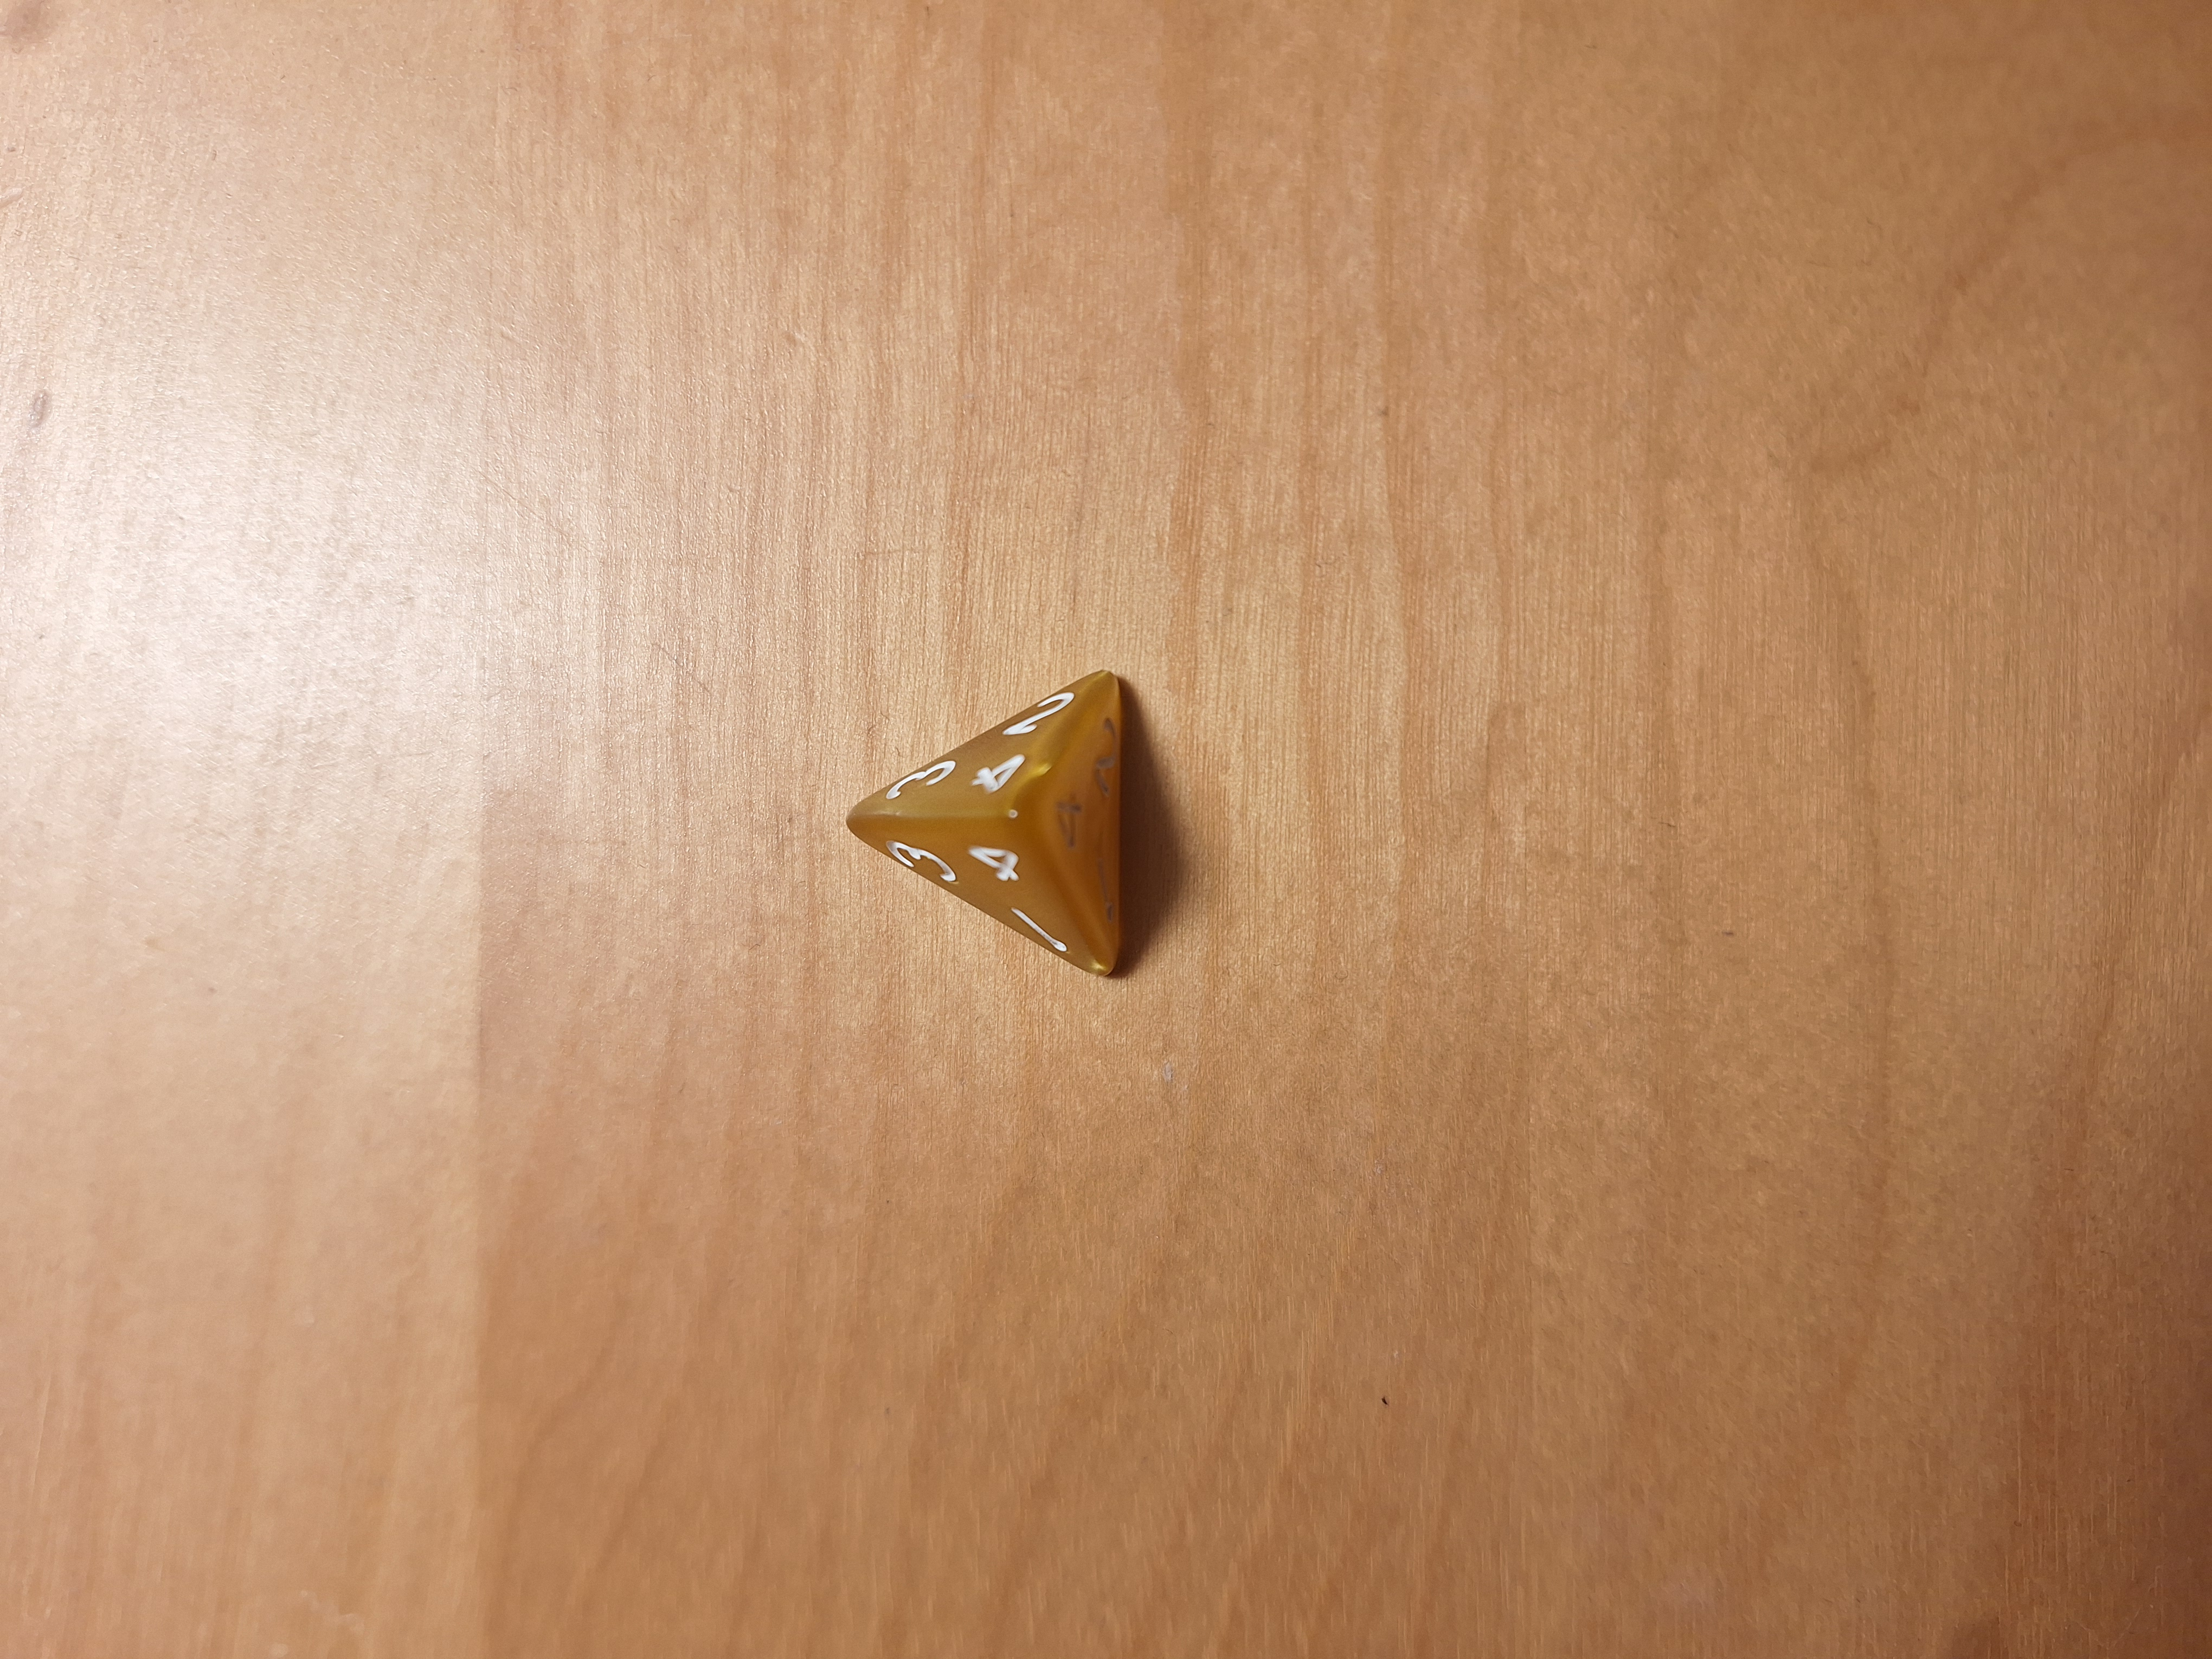
\includegraphics[width=.9\linewidth, trim={250mm 200mm 350mm 150mm}, clip]{chapters/testy/figures/k4.jpg}
        \caption{\label{fig:k4}Kość czterościenna}
      \end{subfigure}%
      \begin{subfigure}{.3\textwidth}
        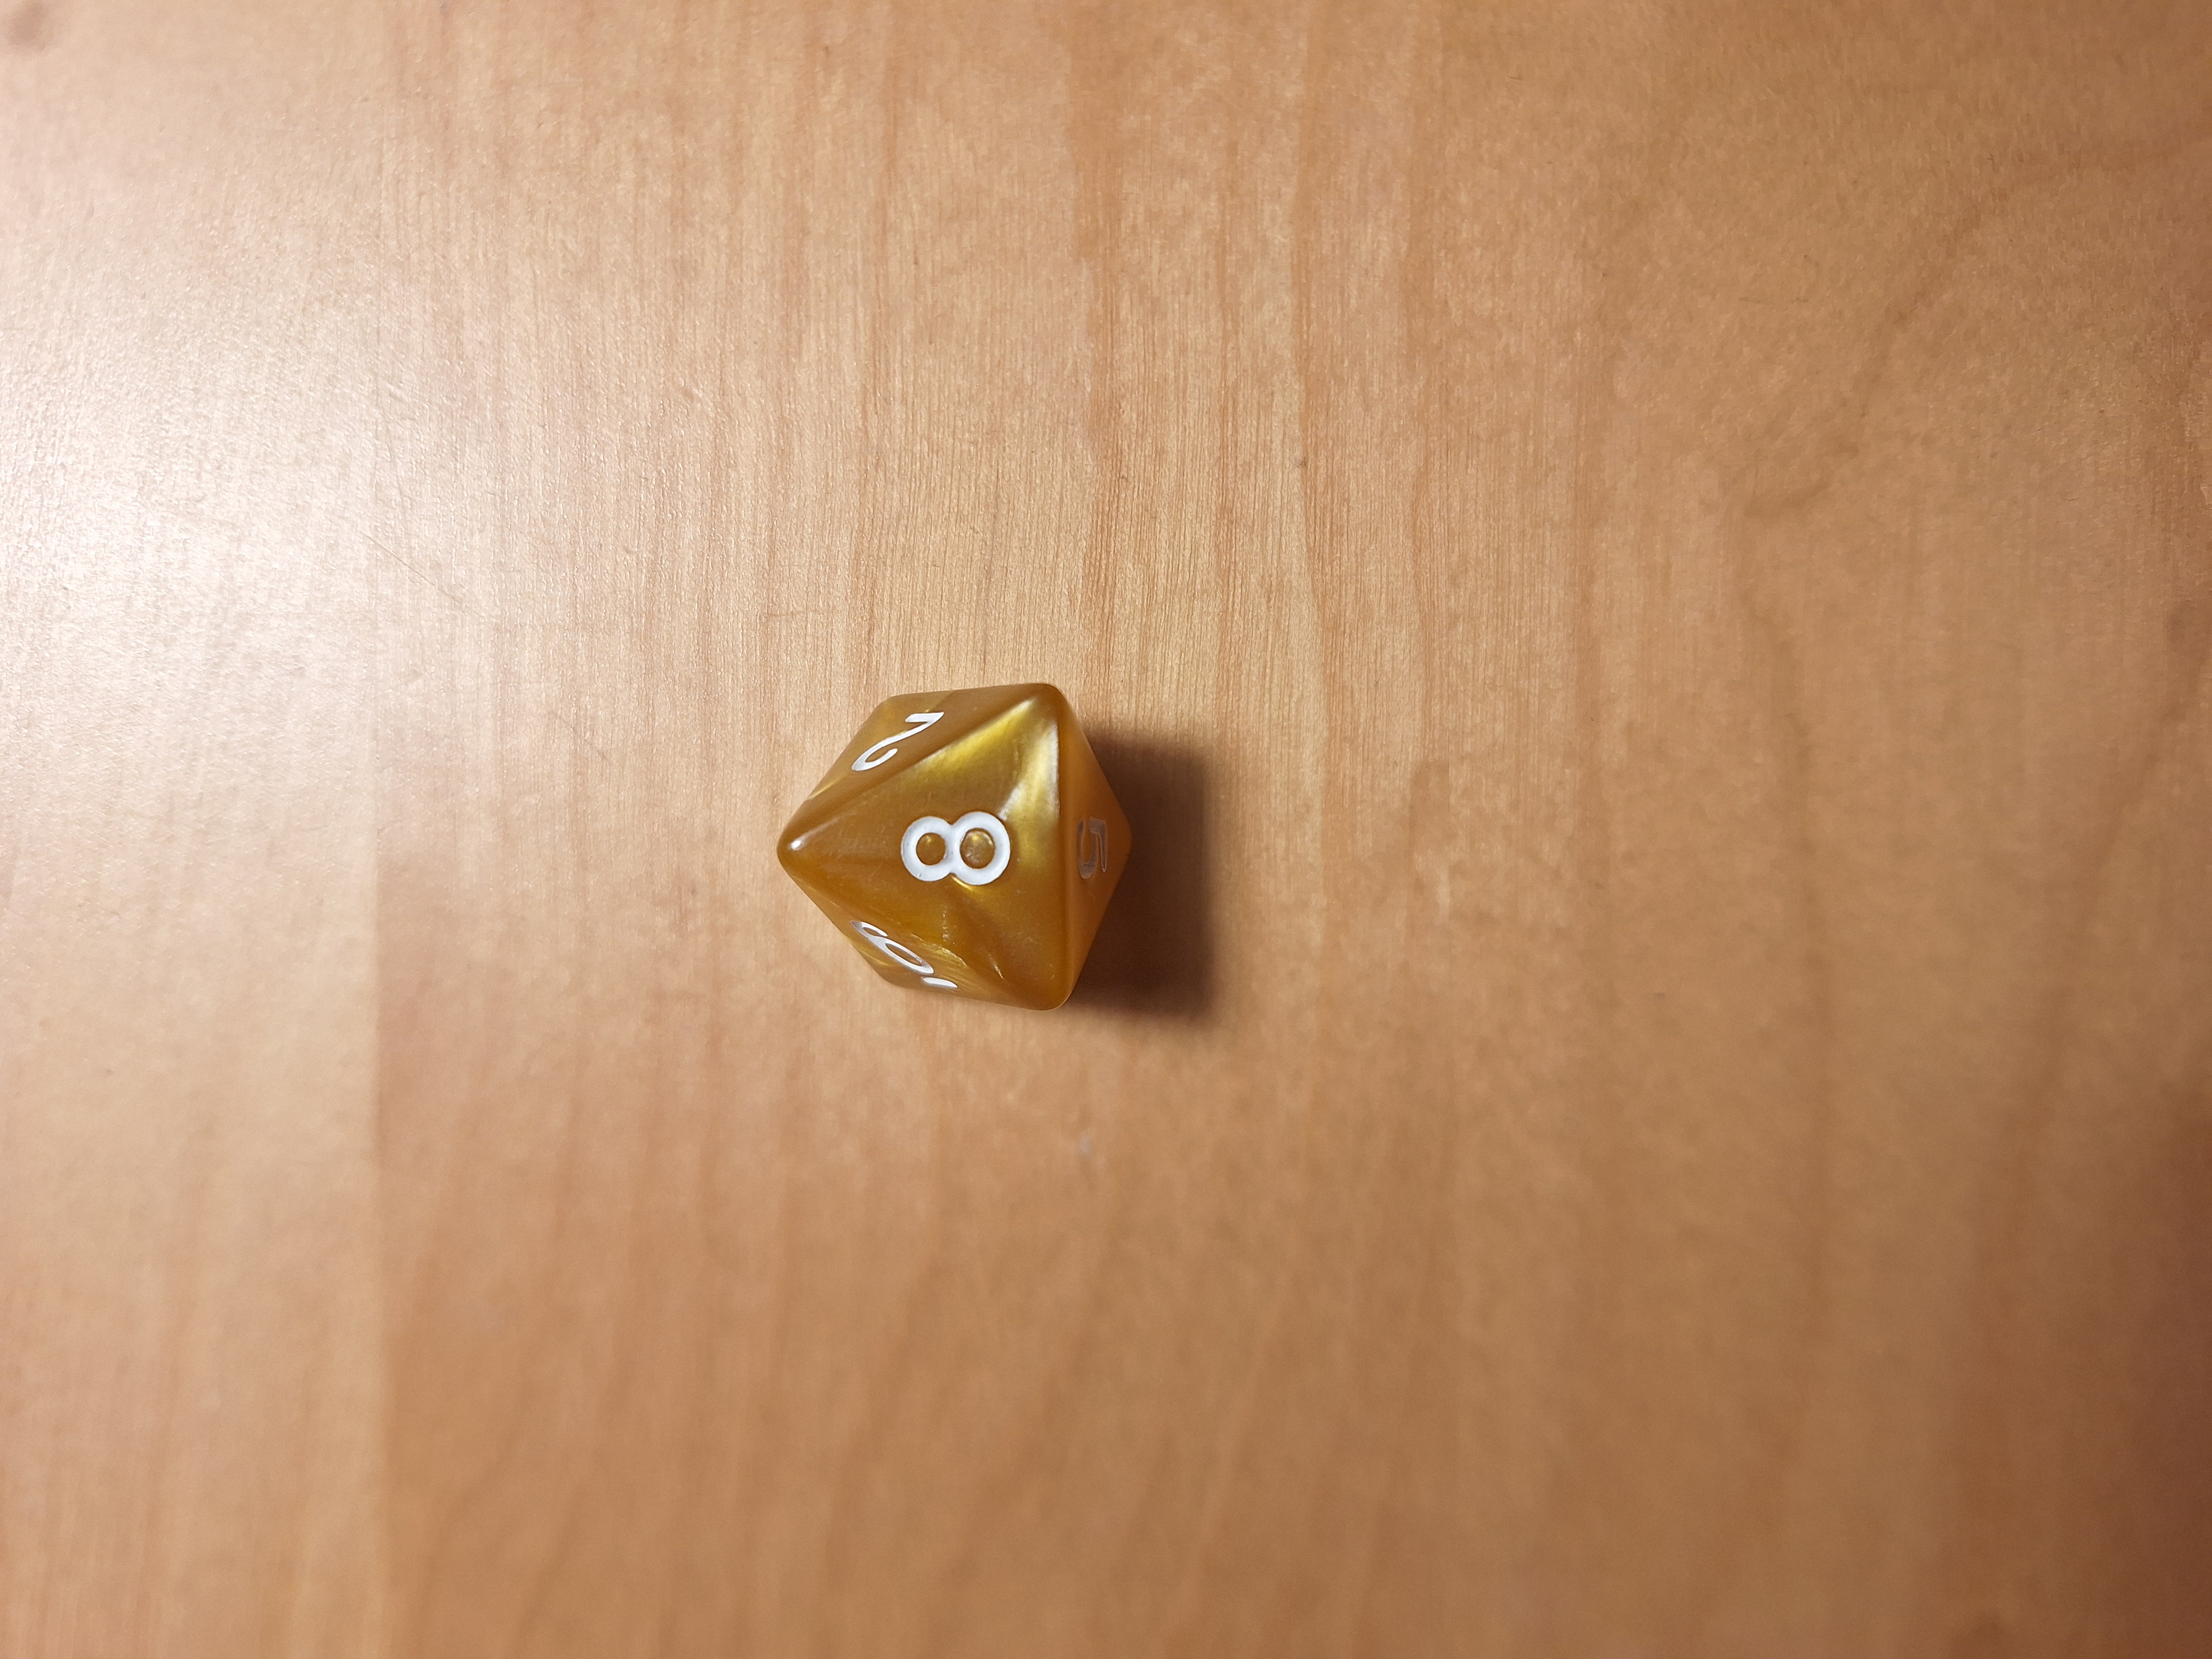
\includegraphics[width=.9\linewidth, trim={250mm 200mm 350mm 150mm}, clip]{chapters/testy/figures/k8.jpg}
        \caption{\label{fig:k8}Kość ośmiościenna}
      \end{subfigure}%
       \begin{subfigure}{.3\textwidth}
        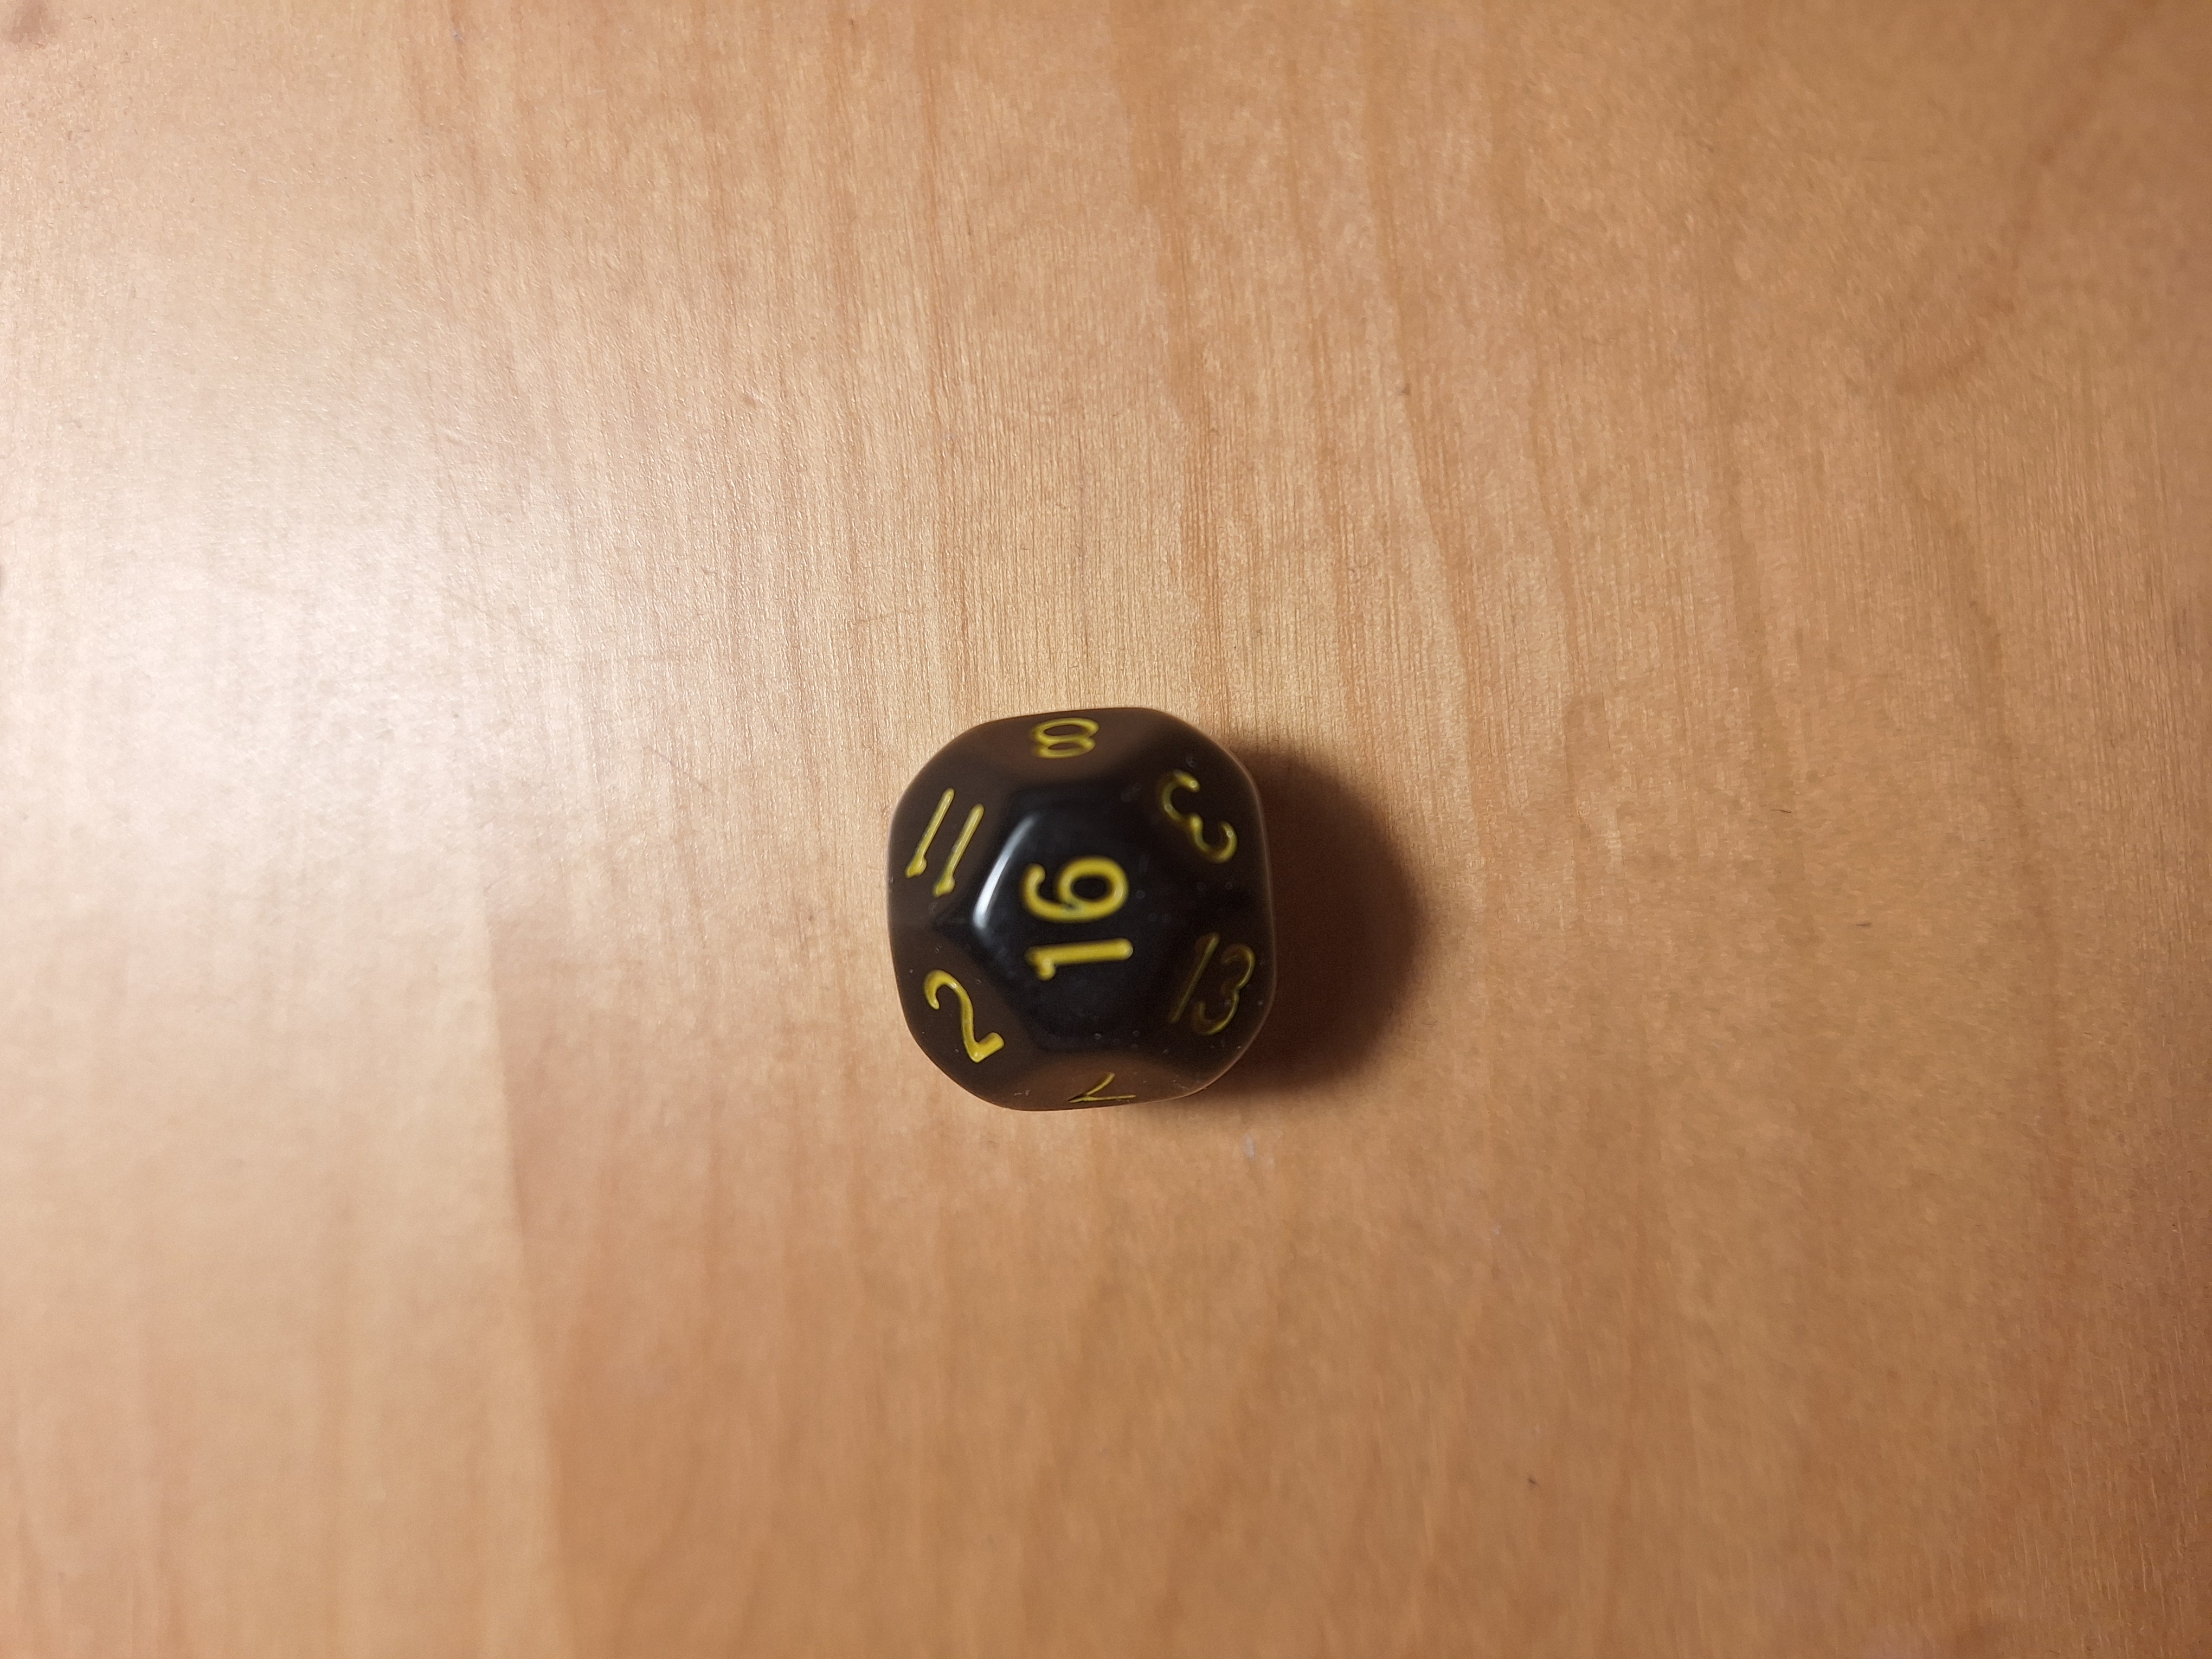
\includegraphics[width=.9\textwidth, trim={300mm 150mm 300mm 200mm}, clip]{chapters/testy/figures/k16.jpg}
        \caption{\label{fig:k16}Kość szesnastościenna}
      \end{subfigure}
    \caption{Zdjęcia kości z góry}
    \end{figure}